\section{Theory}

\subsection{The barotropic Rossby wave equation}

A problem with the current vorticity \cref{eq:QG_vorticity} is
that it is nonlinear, in order obtain linear wave solutions we need to
linearise the equation. We will linearise \cref{eq:QG_vorticity} by supposing
that the flow can be represented by a mean flow plus some small perturbation:
\begin{equation}\label{eq:VeloctiyPertubation}
    \begin{split}
    u = U + u' \quad  |U| >> u' \\
    v = V + v' \quad  |V| >> v'
    \end{split}
\end{equation}
Then the vorticity of the mean flow and the perturbation is:

\begin{equation}\label{eq:VortPertubation}
    Z = \pdv{V}{x} - \pdv{U}{y} \; , \quad \zeta' = \pdv{v'}{x} - \pdv{u'}{y}
\end{equation}

To linearise the Coriolis parameter, we expand $f$
around a reference latitude $\theta_0$,
\begin{equation}\label{eq:Beta_approx}
    f \approx f_0 + \beta y
\end{equation}
where $f_0 = 2\Omega \sin(\theta)$, $\beta = 2\cos (\theta_0)/R_e$ and $R_e$ is
the radius of the earth. This linearisation of the Coriolis parameter
\cref{eq:Beta_approx} is commonly referred to as the $\beta-\mathrm{plane}$
approximation.

Inserting  \cref{eq:Beta_approx} and \cref{eq:VeloctiyPertubation} in to the
vorticity equation \cref{eq:QG_vorticity}.

\begin{equation}
    \pdv{\zeta'}{t} + (U+u')\pdv{\zeta'}{x} + (V+v')\pdv{\zeta'}{y} + \bvec{U}
    \cdot \nabla q_s + u' \pdv{q_s}{x} + v' \pdv{q_s}{y} = 0
\end{equation}
\begin{equation}\label{eq:q_s}
    q_s = Z + f_0 + \beta y
\end{equation}
The mean flow $\bvec{U}$ is geostrophic, consequently the flow will be parallel
to the contours of stationary potential vorticity $q_s$, ergo $\bvec{U} \cdot
\nabla q_s = 0$. The perturbations are assumed to be weak so that perturbations
advecting perturbations can be neglected. Thus we get the following linearised
barotropic vorticity equation:

\begin{equation}
    \pdv{\zeta '}{t} + U\pdv{\zeta'}{x} + V\pdv{\zeta'}{y} + \beta v' = 0
\end{equation}
We will drop the primes from here on. Next we suppose that the velocity of
the mean flow is zero, and express the perturbation velocities in terms of the streamfunction
$\psi$, $u = -\pdv{\psi}{y}$, $v = \pdv{\psi}{x}$ and $\zeta = \nabla_H^2 \psi
$. The equation we end up with is the barotropic Rossby wave equation
\cref{eq:barotropicRossby} in the absence of a mean flow.

\begin{equation}\label{eq:barotropicRossby}
    \pdv{}{t} \nabla_H^2 \psi + \beta \pdv{\psi}{x} = 0
\end{equation}

\subsection{Analytic expression of phase velocities}
Proceeding from the barotropic Rossby wave equation \cref{eq:barotropicRossby}
we will find analytical expression for the phase velocity in
one dimension, first with periodic boundary conditions and then with bounded
boundaries.
\subsubsection{Periodic boundaries}
We assume the following periodic solution \cref{eq:waveSolution}.
At $x=0$ we have $\psi = A\cos{(-\omega t)}$ and at $x = L$, $\psi = A
\cos{(2n\pi -\omega)}$, and because cosine is periodic with a period of $2\pi$,
we see that \cref{eq:waveSolution} satisfies the boundary conditions.
Next we insert \cref{eq:waveSolution} into the barotropic Rossby wave equation
\cref{eq:barotropicRossby}.
\begin{equation}\label{eq:waveSolution}
    \psi = A\cos{(2n\pi x /L - \omega t)}
\end{equation}
Using the one dimensional vorticity $\zeta_x = \pdv{v}{x} = \pdv[2]{\psi}{x}$

\begin{equation}
    \pdv{}{t} \left(-A (2n\pi/L)^2  \cos{(2n\pi x/L - \omega t)}\right) - \beta
     (2n\pi/L) A \sin{(2n x\pi/L - \omega t) = 0}
\end{equation}

\begin{equation}
    -(2n\pi/L)\omega \cancel{A\sin{(2n x\pi/L - \omega t)}} - \beta
    \cancel{A\sin{(2 xn\pi/L - \omega t)}} = 0
\end{equation}

\begin{equation}
    (2n\pi / L) \omega = \beta
\end{equation}

\begin{equation}\label{eq:omega1}
    \omega = \frac{-\beta L}{2n\pi}
\end{equation}

The phase speed of the Rossby wave can be derived by considering the phase of
the wave \cref{eq:phase}.
\begin{equation}\label{eq:phase}
    \theta = \frac{n \pi x}{L} - \omega t
\end{equation}
Then the peak of the wave would be at $\theta = 2\pi$, where $\psi = A\cos{(2\pi)}$.
This peak corresponds to a high pressure point in the flow. To get the motion of this point we can solve
\cref{eq:phase} for x, $x=\theta L / 2n \pi + \omega t L / 2n \pi$ and then
obtaining the phase speed by taking the time derivative.
\begin{equation}
    c = \dv{x}{t} = \frac{\omega L}{2n\pi}
\end{equation}
Inserting the expression for $\omega$ obtained previously \cref{eq:omega1}, we
get the following expression for the phase speed.
\begin{equation}\label{eq:Phase-speed1}
    c = \frac{-\beta}{k^2} = \frac{-\beta L^2}{(2n\pi)^2}
\end{equation}
Then according to \cref{eq:Phase-speed1} the Rossby waves will propagate
toward the west.
\subsubsection{Bounded boundaries}
In the ocean the boundaries would be better represented using bounded boundary
condition. We will suppose a wavelike solution of \cref{eq:barotropicRossby}
where the amplitude of the wave also vary in $x$. We
require there to be no flow at the endpoints, which we can enforce with simple
Dirichlet conditions $\psi= 0$ at $x=0$ and $x=L$.
\begin{equation}\label{eq:waveSolution2}
    \psi = A(x)\cos{(kx-\omega t)}
\end{equation}
Inserting \label{eq:waveSolution2} into the BRWE
\cref{eq:barotropicRossby}, and then differentiating we get the following
equation:

\begin{equation}\label{eq:step1}
    \begin{split}
    \sin{(kx-wt)\left(\omega(A''(x)-k^2A(x))- \beta A(x)\right)} \\
    + \cos{(kx - \omega t)}\left(\omega 2kA'(x) +\beta A'(x)\right) = 0
    \end{split}
\end{equation}
The terms in front of the cosine and sine has to be zero, which means that we
can split equation into two equations, one for the sine and one cosine
terms respectively (\cref{eq:sine-terms}, \cref{eq:cos-terms}).

\begin{equation}\label{eq:sine-terms}
    \omega A''(x) -\omega k^2 A(x) - \beta A(x) = 0
\end{equation}
\begin{equation}\label{eq:cos-terms}
    \omega 2 k A'(x) + \beta A'(x) = 0
\end{equation}
Solving the equation for the cosine terms \cref{eq:cos-terms} with respect to
$\omega$:
\begin{equation}
    \omega = -\frac{\beta}{2k}
\end{equation}
Inserting the expression for omega into \cref{eq:sine-terms} and solving the ODE
gives us the following expression for $A(x)$
\begin{equation}\label{eq:A_x}
    A(x) = C_1 \cos{(kx) + C_2 \sin{(kx)}}
\end{equation}
Imposing the boundary condition at $x=0$ requires $C_1$ to be zero, ruling
out the cosine term in \cref{eq:A_x}. Imposing the boundary condition $\psi=0$
at $x=L$ yields the following expression for A(x).
\begin{equation}
    A(x) = \sin{\left(\frac{n\pi}{L} x \right)}
\end{equation}
Then final solution becomes:
\begin{equation}
    \psi(x,t) = \sin{\left(\frac{n\pi}{L} x \right)} \cos{(kx - \omega t)}
\end{equation}
The solution contains the same cosine term as in the periodic domain, but is now
modulated by a sine term that enforces the boundary conditions and increases
the number of throughs and ridges compared to the periodic solution.
The phase speed can be calculated in the same manner as in the periodic case,
except now $k=\frac{n\pi}{L}$.

\begin{equation}
    c = \dv{x}{t} = \frac{\omega}{k} = -\frac{\beta}{2k^2} = -\frac{\beta L^2}{2
    \pi^2 n^2}
\end{equation}
The phase speed for the Rossby waves with solid boundaries is twice compared to
the periodic boundaries.

\section{Numerical model}


\subsection{Scaling}
Before we do the discretisation it is useful to nondimensionalise the BRWE.
We scale the BRWE using $x = \tilde{x} L $ and $t = \frac{\tilde{t}}{L \beta}$.
The dimensionless phase speed is then $\frac{d\tilde{x}}{d\tilde{t}} = \frac{1}
{\beta L^2} c$. For wavenumber two this gives us phase speeds of
$-0.0063$ for the periodic case and $c = -0.012665$ for the bounded case.
After doing the scaling we end up with the following dimensionless BRWE
\cref{eq:scaled_BRWE}.

\begin{equation}\label{eq:scaled_BRWE}
  \pdv{\zeta}{\tilde{t}} + \pdv{\psi}{\tilde{x}} = 0
\end{equation}


\subsection{Algorithm and finite differences}

The general algorithm for solving the BRWE is outlined in
\cref{algo:vort}.

\begin{algorithm}[H]
  \SetAlgoLined
  initialize $\zeta$ and $\psi$ using sine or gaussian\\
  \For{t=0; t<\text{timesteps}; t++}{
    advance $\zeta$ one timestep \\
    update $\psi$ using jacobis method
  }
  \caption{General algorithm for solving the BRWE.}
  \label{algo:vort}
\end{algorithm}

We implemented two methods for advancing $\zeta$ using centered
(\cref{eq:centered}) and forward (\cref{eq:forward}) differences. For the
planetary vorticity advection term we used centered differences. This lead to
the forward time centered space (FTCS) \cref{eq:advance_centered} and centered
time centered space (CTCS) \cref{eq:advance_forward} schemes.


\begin{equation} \label{eq:centered}
  \pdv{\zeta}{t} \approx \frac{\zeta_{}^{n+1} - \zeta_{}^{n-1}}{2 \Delta t}
\end{equation}

\begin{equation} \label{eq:forward}
  \pdv{\zeta}{t} \approx \frac{\zeta_{}^{n+1} - \zeta_{}^{n}}{\Delta t}
\end{equation}


\begin{equation} \label{eq:advance_centered}
  \zeta_{i}^{n+1} = \zeta_{i}^{n-1} - \frac{\Delta t}{2 \Delta x}
    (\psi_{i+1}^{n} - \psi_{i-1}^{n})
\end{equation}


\begin{equation}   \label{eq:advance_forward}
  \zeta_{i}^{n+1} = \zeta_{i}^{n} - \frac{\Delta t}{\Delta x} (\psi_{i+1}^{n} - \psi_{i-1}^{n})
\end{equation}

The truncation error of the centered difference terms are of order
$(\Delta x)^2$ and
$(\Delta t)^2$, while the forward difference term are of order $\Delta t$
 \parencite{langtangen}.


\subsection{Initalization}

We will test different initial condition for $\psi$. In one dimension we will
use the sinusoidal $\psi(x, 0) = \sin{(4 \pi x)}$ and Gaussian $\psi(x, 0) =
\exp{-\para{\frac{x - x_0}{\sigma}}^2}$.
In two dimensions we will use a two-dimensional sinusoidal $\psi(x,y,0) =
\sin{(4 \pi x)} \sin{(4 \pi y)}$. $ \zeta(t=0) $ was initalized as $
\pdv[2]{\psi}{x} $ in one dimension and as $\nabla_H^2 \psi$ in two dimensions.

For CTCS $\zeta_{j}^{1}$ is a function of $\zeta_{j}^{-1}$ which we don't know.
We could either set $\zeta_{j}^{-1} = \zeta_{j}^{0}$ or use the FTCS scheme
backwards. At first we tried to implement the latter but ran into problems we
could not resolve, and opted for the first option.

\subsection{Jacobis method}

After advancing the vorticity one timestep we adjust the stream function
according to $\zeta = \nabla_H^2 \psi$.  We do this by solving the poisson
equation using
jacobis method. Jacobis method requires a convergence parameter for deciding
when to stop iterating. To determine this parameter we tested our
numerical solutions  against two analytical solutions
of poissons equation, one bounded and one periodic.

\begin{figure}[h]
  \centering
  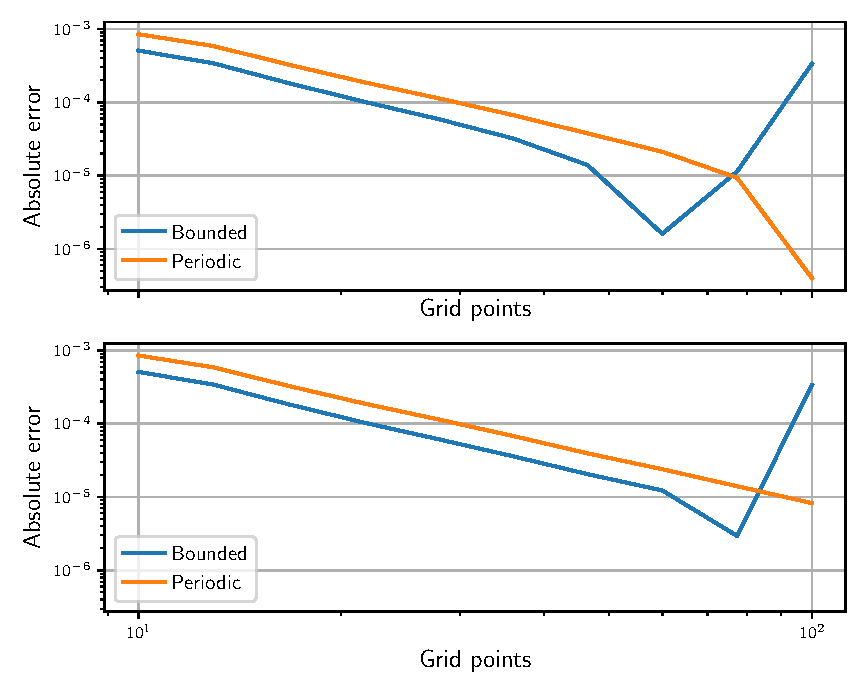
\includegraphics[width=\textwidth]{../figures/error_jacobi.pdf}
  \caption{Absolute error of jacobis method
  compared to analytical solutions of poissons equation. Convergence parameter set to (from top to bottom) 10$^{-6}$, 10$^{-8}$ and 10$^{-10}$.
  The absolute error should have a slope of -2 in loglog space since we use
  a centered second order scheme with truncation error proportional to $(\Delta x)^2$.
  The larger values of the convergence parameter has the correct slope for small
  grids, but performs worse with larger grids. As the parameter is lowered the
  slope is correct for increasingly larger grids.}
  \label{fig:error_jacobi}
\end{figure}

\Cref{fig:error_jacobi}
shows the absolute error of jacobis method compared to the analytical solutions.
For small convergence parameters, Jacobis method gives a smaller
absolute error on large grids.
For our model runs we will be using close to 40 grid points and we found that
Jacobis method achieved satisfactory result when setting the convergence
parameter to 10$^{-8}$.

\subsection{Stability and comparison of timestepping methods}

To assess the stability of the two timestepping methods we can insert solutions
of $\psi_{j}^{n} = A^n e^{ikj \Delta x}$ into the FTCS and CTCS schemes.
For both schemes we need to use that
$\pdv{\zeta}{t} = -k^2 \pdv{\psi}{t} = - \frac{1}{c} \pdv{\psi}{t}$

\subsubsection{FTCS}
The FTCS gives,
\begin{align}
  &-\frac{1}{c} \frac{A^{n+1} e^{ikj\Delta x} - A^n e^{ikj\Delta x}}{\Delta t} + \frac{A^n e^{ik(j+1)\Delta x} - A^n e^{ik(j-1)\Delta x}}{2\Delta x} \\
  &= A^n e^{ikj} \brak{A - 1 - c\frac{\Delta t}{2 \Delta x} \para{e^{ik\Delta x} - e^{-ik\Delta x}}} = 0
\end{align}

Solving for A leads to $ A = 1 + \frac{c \Delta t}{\Delta x} sin(k\Delta x) i$.
For the numerical solution to stay stable we need $\abs{A}^2 <= 1$, which can
not be satisfied. Therefore the FTCS scheme is unconditionally unstable. The
instability of the FTCS scheme is shown in \cref{fig:compare_small}, where we
see the FTCS solutions diverging around t=10. The oscillations might be caused
by our lack of initalizing $\zeta_{j}^{-1}$ properly. Another view of the
instability is given in \cref{sec:stability} which shows the whole wave.

\begin{figure}[h]
  \centering
  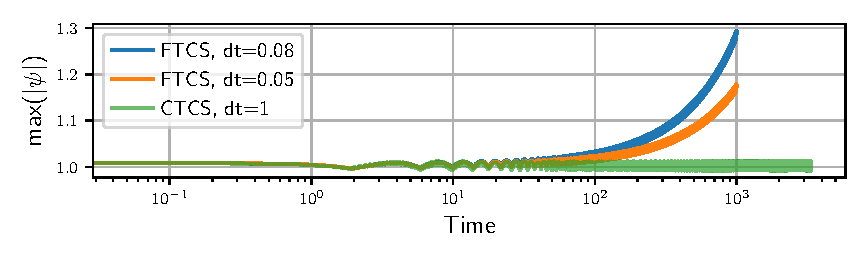
\includegraphics[width=\textwidth]{../figures/stability_compare.pdf}
  \caption{Comparison of maximum value of $\psi$ as a function of time with
  different timesteps and schemes.
  The CTCS scheme with a long timestep seems stable, while FTCS with small timesteps
  both diverges at around t=10.}
  \label{fig:compare_small}
\end{figure}


\subsubsection{CTCS}

For the CTCS scheme we get,
\begin{align}
  &-\frac{1}{c}\frac{A^{n+1} e^{ikj\Delta x} - A^{n-1} e^{ikj \Delta x}}{2 \Delta t} + \frac{A^n e^{ik(j+1) \Delta x} - A^{n} e^{ik(j-1)\Delta x}}{2 \Delta x} \\
  &= A^n e^{ikj\Delta x} \brak{ A - A^{-1} - c\frac{\Delta t}{\Delta x} \para{2 sin(k\Delta x) i}} = 0
\end{align}

Setting $c\frac{\Delta t}{\Delta x} = \alpha$ and solving for A gives
$ A = \alpha sin(k\Delta x) i \pm \sqrt{-\alpha^2 sin(k\Delta x)^2 + 1}$.
This gives us two cases, $\abs{\alpha} > 1$ and $\abs{\alpha} \leq 1$
For $\abs{\alpha} < 1$ we get
$\abs{A}^2 = \alpha^2 sin(k\Delta x) + 1 - \alpha^2 sin(k\Delta x) = 1$
which is unconditionally stable.
For $\abs{\alpha} > 1$ we get $\abs{A}^2 = \para{ \alpha sin(k\Delta x) \pm
\sqrt{\alpha^2 sin(k\Delta x)^2 -1 }}^2$ which will be unstable for some
combinations of k and $\Delta x$.
We therefore find the stability criterion for the CTCS scheme to be
$ \frac{\Delta t}{\Delta x} < \frac{1}{c} = k^2$.

For the CTCS scheme with a sinusoidal inital state with wavenumber $4 \pi$ and
$\Delta x = \frac{1}{40}$
this corresponds to having $ \Delta t \leq \frac{\para{4 \pi}^2}{40} = 3.948$.
Some runs with periodic boundaries is shown in \cref{fig:compare_ctcs}.


\begin{figure}[h]
  \centering
  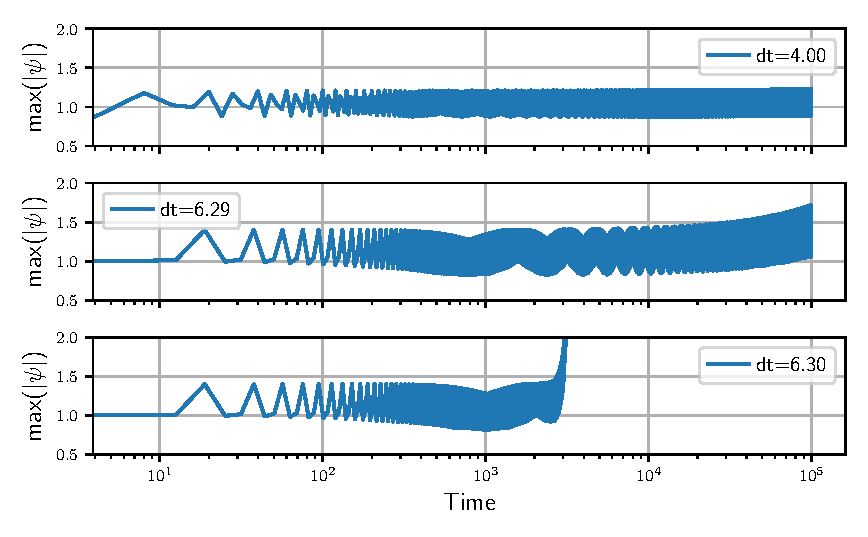
\includegraphics[width=\textwidth]{../figures/stability_ctcs.pdf}
  \caption{Comparison of maximum value of $\psi$ as a function of time with
  different timesteps.
  The top figure is barely outside of the stability criterion and was not run
  long enough to show any instability. The two bottom figures have very similar
  timesteps but shows signs off instability at very different times.}
  \label{fig:compare_ctcs}
\end{figure}
